\documentclass{standalone}

\usepackage{times}
\usepackage{amsmath}
\usepackage{amssymb}

\usepackage[dvipsnames]{xcolor}
\usepackage{tikz}
\usetikzlibrary{arrows,backgrounds,scopes}

\usepackage{pgfplots}
\pgfplotsset{compat=1.15}

\definecolor{red}{HTML}{cf555a}

\begin{document}
	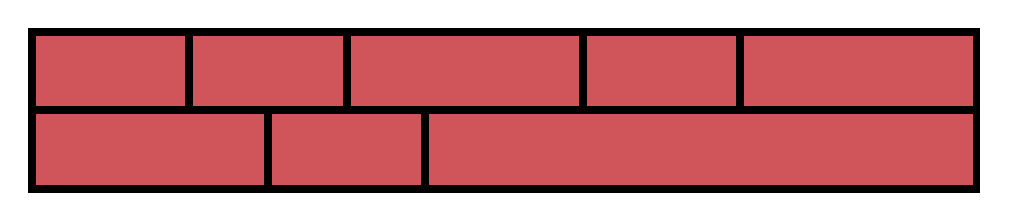
\begin{tikzpicture}[line width=0.1cm]
		\draw[fill=red] (0,0) rectangle(3,1);
		\draw[fill=red] (3,0) rectangle(5,1);
		\draw[fill=red] (5,0) rectangle(12,1);
		
		
		\draw[fill=red] (0,1) rectangle(2,2);
		%\draw[fill=red] (2,1) rectangle(9,2);
		\draw[fill=red] (2,1) rectangle(4,2);
		\draw[fill=red] (4,1) rectangle(7,2);
		\draw[fill=red] (7,1) rectangle(9,2);
		\draw[fill=red] (9,1) rectangle(12,2);
	\end{tikzpicture}
\end{document} 
